
% spellcheck: ok
% mikes: ok

% ============================================================
\chapter{Simulations}{}{}
\label{ch:simulation}

\index{data analysis!simulations|(}
\index{simulations|(}
  
% In this chapter we look at simulations as a way to understand data.
% This chapter therefore straddles the previous part (on Modeling) and
% the current one (on Computation): an important part in every
% simulation is setting up the \emph{simulation model}, that is the
% abstract and often simplified description of the actual events that
% is used to construct the executable simulation code. But the emphasis
% falls quite naturally on running the simulations, and hence this 
% chapter is properly to be found in the part on Computational issues.

\Fint{In this chapter, we look at simulations as a way to understand data.
It may seem strange to find} simulations included in a book on data
analysis: don't simulations just generate even \emph{more} data that
needs to be analyzed? Not necessarily---as we will see, simulations in
the form of \emph{resampling methods} provide a family of techniques
for extracting information from data. In addition, simulations can be
useful when developing and validating models, and in this way, they
facilitate our understanding of data. Finally, in the context of this
chapter we can take a brief look at a few other relevant topics, such
as discrete event simulations and queueing theory.

A technical comment: I assume that your programming environment
includes a random-number generator---not only for uniformly
distributed random numbers but also for other distributions (this is a
pretty safe bet). I also assume that this random-number generator
produces random numbers of sufficiently high quality. This is probably
a reasonable assumption, but there's no guarantee: although the theory
of random-number generators is well understood, broken implementations
apparently continue to ship. Most books on simulation methods will
contain information on random-number generators---look there if you
feel that you need more detail.

% ============================================================
\section{A Warm-Up Question}

\index{simulations!about} 

As a warm-up to demonstrate how simulations can help us analyze data,
consider the following example. We are given a data set with the
results of eight tosses of a coin: six Heads and two Tails. Given this
data, would we say the coin is biased?\vfill\pagebreak

The problem is that the data set is small---if there had been 80,000
tosses of which 60,000 came out Heads, then we would have no doubt
that the coin was biased. But with just eight tosses, it seems
plausible that the imbalance in the results might be due to chance
alone---even with a fair coin.

It was for precisely this kind of question that formal statistical
methods were developed. We could now either invoke a classical
frequentist point of view and calculate the probability of obtaining
six or more Heads in eight tosses of a fair coin (\ie, six or more
successes in eight Bernoulli trials with $p=0.5$). The probability
comes out to $37/256 \approx 0.14$, which is not enough to ``reject the
null hypothesis (that the coin is fair) at the 5 percent level.''
Alternatively, we could adopt a Bayesian viewpoint and evaluate the
appropriate likelihood function for the given data set with a
noninformative prior (see Figure \ref{fig:simulation1}). The graph
suggests that the coin is not balanced.

\begin{figure}
  \centerline{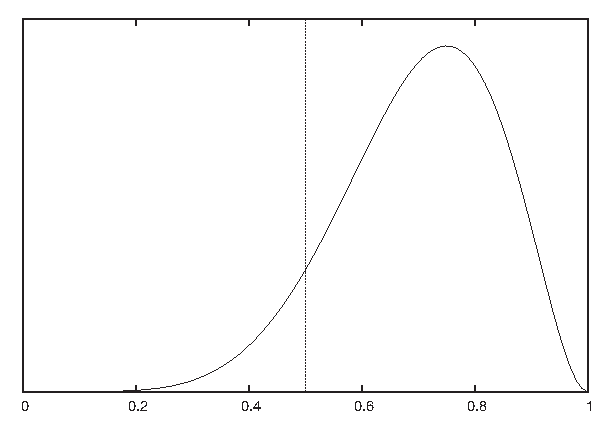
\includegraphics{img/simulation1}}
  \caption{The likelihood function $p^6 (1-p)^2$ of observing six
    Heads and two Tails in eight tosses of a coin, as a function of
    the coin's ``balance parameter'' $p$.}
  \label{fig:simulation1}
\end{figure}

But what if we have forgotten how to evaluate either quantity, or
(more likely!)  if we are dealing with a problem more intricate than
the one in this example, so that we neither know the appropriate model to
choose nor the form of the likelihood function? Can we find a quick
way to make progress on the question we started with?

Given the topic of this chapter, the answer is easy. We can
\emph{simulate} tosses of a coin, for various degrees of imbalance,
and then compare the simulation results to our data set.

\begin{verbatim}
import random

repeats, tosses = 60, 8
\end{verbatim}
\begin{verbatim}

def heads( tosses, p ):
    h = 0
    for x in range( 0, tosses ):
        if random.random() < p: h += 1
    return h

p = 0
while p < 1.01:
    for t in range( 0, repeats ):
        print p, "\t", heads( tosses, p )
    p += 0.05
\end{verbatim}

The program is trivial to write, and the results, in the form of a
jitter plot, are shown in Figure \ref{fig:simulation2}. (For each
value of the parameter $p$, which controls the imbalance of the coin,
we have performed 60 repeats of 8 tosses each and counted the number
of Heads in each repeat.)

\begin{figure}
  \centerline{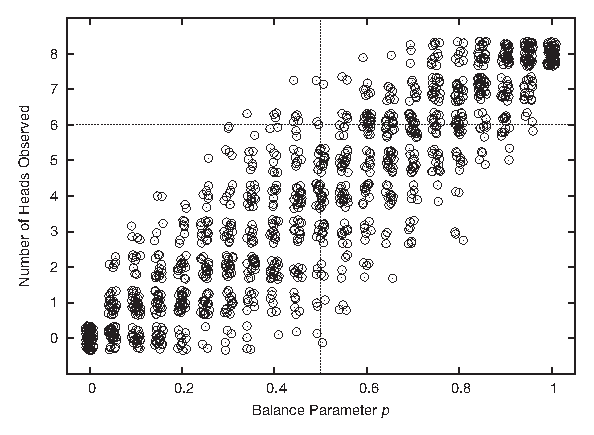
\includegraphics{img/simulation2}}
  \caption{Results of 60 simulation runs, each consisting of eight tosses
    of a coin, for different values of the coin's ``balance
    parameter'' $p$.  Shown are the number of Heads observed in each
    run.  Although a slight balance toward Heads ($p \approx 0.7$)
    seems most probable, note that as many as six Heads can
    occasionally be observed even with a coin that is balanced toward
    Tails.}
  \label{fig:simulation2}
\end{figure}

The figure is quite clear: for $p=0.5$ (\ie, a balanced coin), it is
pretty unlikely to obtain six or more Heads, although not at all
impossible. On the other hand, given that we have observed six Heads,
we would expect the parameter to fall into the range $p=0.6, \dots,
0.7$.  We have thus not only answered the question we started with but
also given it some context. The simulation therefore not only helped
us understand the actual data set but also allowed us to explore the
system that produced it. Not bad for 15 lines of code.


% ============================================================
\section{Monte Carlo Simulations}

\index{simulations!Monte Carlo simulations|(}
\index{Monte Carlo simulations|(}
  
The term \emph{Monte Carlo simulation} is frequently used to describe
any method that involves the generation of random points as input for
subsequent operations.

Monte Carlo techniques are a major topic all by themselves. Here, I
only want to sketch two applications that are particularly relevant in
the context of data analysis and modeling. First, simulations allow us
to verify analytical work and to experiment with it further; second,
simulations are a way of obtaining results from models for which
analytical solutions are not available.

% Combinatorial problems arise frequently in probabilistic modeling ---
% the case study in chapter \ref{unk} is an example. Although one can
% often work out an exact solution for simple scenarios, even slightly
% more general problems are often infeasible (or at least impractical).
% 
% - verify analytical work
% - verify that the assumptions going into the model are correct
% - make fewer artificial assumptions
% - do what-if calculations on the ``model''


\subsection{Combinatorial Problems}

\index{Monte Carlo simulations!combinatorial problems|(}
\index{combinatorial problems} 

Many basic combinatorial problems can be solved exactly---but
obtaining a solution is often difficult.  Even when one is able to
find a solution, it is surprisingly easy to arrive at incorrect
conclusions, missing factors like $1/2$ or $1/n!$ and so on.  And
lastly, it takes only innocuous looking changes to a problem
formulation to render the problem intractable.

In contrast, simulations for typical combinatorial problems are often
trivially easy to write. Hence they are a great way to validate
theoretical results, and they can be extended to explore problems that
are not tractable otherwise.

Here are some examples of questions that can be answered easily in
this way:

\begin{itemize}
\item If we place $n$ balls into $n$ boxes, what is the probability
  that no more than two boxes contain two or more balls? What if I
  told you that \emph{exactly} $m$ boxes are empty? What if \emph{at
    most} $m$ boxes are empty?

\item If we try keys from a key chain containing $n$ different keys,
  how many keys will we have to try before finding the one that fits
  the lock? How is the answer different if we try keys randomly (with
  replacement) as opposed to in order (without replacement)?

\item Suppose an urn contains $2 n$ tokens consisting of $n$ pairs of
  items. (Each item is marked in such a way that we can tell to which
  pair it belongs.) Repeatedly select a single token from the urn and
  put it aside. Whenever the most recently selected token is the
  \emph{second} item from a pair, take both items (\ie, the entire
  pair) and return them to the urn. How many ``broken pairs'' will you
  have set aside on average? How does the answer change if we care
  about triples instead of pairs? What fluctuations can we expect
  around the average value?
\end{itemize}

The last problem is a good example of the kind of problem for which
the simple case (average number of broken pairs) is fairly easy to
solve but that becomes rapidly more complicated as we make seemingly
small modifications to the original problem (\eg, going from pairs to
triples). However, in a simulation such changes do not pose any
special difficulties.

Another way that simulations can be helpful concerns situations that
appear unfamiliar or even paradoxical. Simulations allow us to
\emph{see} how the system behaves and thereby to develop intuition for
it. We already encountered an example in the Workshop section of
Chapter \ref{ch:probability}, where we studied probability
distributions without expectation values. Let's look at another
example.

Suppose, we are presented with a choice of three closed envelopes. One
envelope contains a prize, the other two are empty. After we have
selected an envelope, it is revealed that one of the envelopes that we
had \emph{not} selected is empty. We are now permitted to choose
again.  What should we do? Stick with our initial selection? Randomly
choose between the two remaining envelopes? Or pick the remaining
envelope---that is, not the one that we selected initially and not the
one that has been opened?

This is a famous problem, which is sometimes known as the ``Monty Hall
Problem'' (after the host of a game show that featured a similar game).

As it turns out, the last strategy (always switch to the remaining
envelope) is the most beneficial. The problem appears to be
paradoxical because the additional information that is revealed (that
an envelope we did not select is empty) does not seem to be useful in
any way. How can this information affect the probability that our
initial guess was correct?

The argument goes as follows. Our initial selection is correct with
probability $p = 1/3$ (because one envelope among the original three
contains the prize). If we stick with our original choice, then we
should therefore have a 33 percent chance of winning.  On the other
hand, if in our second choice, we choose randomly from the remaining
options (meaning that we are as likely to pick the initially chosen
envelope or the remaining one), then we will select the correct
envelope with probability $p = 1/2$ (because now one out of two
envelopes contains the prize). A random choice is therefore better
than staying put!

But this is still not the best strategy. Remember that our initial
choice only had a $p = 1/3$ probability of being correct---in other
words, it has probability $q = 2/3$ of being \emph{wrong}. The
additional information (the opening of an empty envelope) does not
change this probability, but \emph{it removes all alternatives}. Since
our original choice is wrong with probability $q = 2/3$ and since now
there is only one other envelope remaining, switching to this
remaining envelope should lead to a win with 66 percent probability!

I don't know about you, but this is one of those cases where I had to
``see it to believe it.'' Although the argument above seems
compelling, I still find it hard to accept. The program in the
following listing helped me do exactly that.

\begin{verbatim}
import sys
import random as rnd

strategy = sys.argv[1]   # must be 'stick', 'choose', or 'switch'

wins = 0
for trial in range( 1000 ):    
\end{verbatim}
\begin{verbatim}
    # The prize is always in envelope 0 ... but we don't know that!
    envelopes = [0, 1, 2]

    first_choice = rnd.choice( envelopes )

    if first_choice == 0:
        envelopes = [0, rnd.choice( [1,2] ) ] # Randomly retain 1 or 2
    else:
        envelopes = [0, first_choice] # Retain winner and first choice

    if strategy == 'stick':
        second_choice = first_choice
    elif strategy == 'choose':
        second_choice = rnd.choice( envelopes )
    elif strategy == 'switch':
        envelopes.remove( first_choice )
        second_choice = envelopes[0]

    # Remember that the prize is in envelope 0
    if second_choice == 0:
        wins += 1

print wins
\end{verbatim}

The program reads our strategy from the command line: the possible
choices are \texttt{stick}, \texttt{choose}, and \texttt{switch}. It
then performs a thousand trials of the game. The ``prize'' is always
in envelope \texttt{0}, but we don't know that. Only if our second
choice equals envelope \texttt{0} we count the game as a win.

The results from running this program are consistent with the argument
given previously: \texttt{stick} wins in one third of all trials,
\texttt{choose} wins half the time, but \texttt{switch} amazingly wins
in two thirds of all cases.

\index{Monte Carlo simulations!combinatorial problems|)}

\subsection{Obtaining Outcome Distributions}

\index{Monte Carlo simulations!outcome distributions|(}
\index{distributions!Monte Carlo simulation outcome distributions|(}
  
Simulations can be helpful to verify with combinatorial problems, but
the primary reason for using simulations is that they allow us to
obtain results that are not available analytically. To arrive at an
analytical solution for a model, we usually have to make simplifying
assumptions. One particularly common one is to replace all random
quantities with their most probable value (the mean-field
approximation; see Chapter \ref{ch:scaling}). This allows us to solve
the model, but we lose information about the distribution of outcomes.
Simulations are a way of retaining the effects of randomness when
determining the consequences of a model.

% To formulate analytical models of the form that we discussed in
% chapters \ref{ch:scaling} and \ref{ch:probability} and to make them
% tractable required us to develop a simplified description, which only
% retained the most essential information. One common strategy in this
% regard is to replace all random quantities by their most probable
% value: of course, this simplifies the problem greatly, but all
% information about the range over which outcomes can vary has been
% lost.
% 
% There are ways to work around this limitation: we can determine by how
% much the inputs typically vary, and then repeat the calculation,
% performing it not only for the most probable value, but also for the
% upper and lower bound on the input quantities. This will give us a
% sense for the bounds on the outcomes, but certainly not their full
% distribution.  Furthermore, working with a single value (be it the
% most probable or some other representative value) instead of the full
% distribution of values is only an approximation.
% 
% By contrast, in a simulation we generate individual points from the
% full distribution of inputs and carry out all operations with the
% individual points. We can then study the set of results to determine
% the distribution of outcomes. In this way, we don't just obtain the
% most probable outcome, but also gain insight into the full
% \emph{range} of outcomes and their respective probabilities.

Let's return to the case study discussed at the end of Chapter
\ref{ch:probability}. We had a visitor population making visits to a
certain website.  Because individual visitors can make repeat visits,
the number of \emph{unique} visitors grows more slowly than the number
of \emph{total} visitors. We found an expression for the number\vadjust{\pagebreak} of
unique visitors over time but had to make some approximations in
order to make progress.  In particular, we assumed that the number of
total visitors per day would be the same every day, and be equal to
the average number of visitors per day. (We also assumed that the
fraction of actual repeat visitors on any given day would equal the
fraction of repeat visitors in the total population.)

Both of these assumptions are of precisely the nature discussed 
earlier: we replaced what in reality is a random quantity with its
most probable value. These approximations made the problem tractable,
but we lost all sense of the accuracy of the result. Let's see how
simulations can help provide additional insight to this situation.

The solution which in Chapter \ref{ch:probability} was a \emph{model}:
an analytical (mean-field) model.  The short program that follows is
another model of the same system, but this time it is a
\emph{simulation model}. It is a model in the sense that again
everything that is not absolutely essential has been stripped away:
there is no website, no actual visits, no browsing behavior. But the
model retains two aspects that are important and that were missing
from the mean-field model. First, the number of visitors per day is no
longer fixed, instead it is distributed according to a Gaussian
distribution.  Second, we have a notion of individual visitors (as
elements of the list \texttt{has\_visited}), and on every ``day'' we
make a random selection from this set of visitors to determine who
does visit on this day and who does not.

\begin{verbatim}
import random as rnd

n = 1000    # total visitors
k = 100     # avg visitors per day
s = 50      # daily variation

def trial():
    visitors_for_day = [0]  # No visitors on day 0

    has_visited = [0]*n     # A flag for each visitor
    for day in range( 31 ):
        visitors_today = max( 0, int(rnd.gauss( k, s )) )

        # Pick the individuals who visited today and mark them 
        for i in rnd.sample( range( n ), visitors_today ):
            has_visited[i] = 1  

        # Find the total number of unique visitors so far
        visitors_for_day.append( sum(has_visited) )

    return visitors_for_day
    
    
for t in range( 25 ):
    r = trial()
    for i in range( len(r) ):
        print i, r[i]

    print
    print
\end{verbatim}

The program performs 25 trials, where each trial consists of a full,
31-day month of visits. For each day, we find the number of visitors
for that day (which must be a positive integer) and then randomly
select the same number of ``visitors'' from our list of visitors,
setting a flag to indicate that they have visited. Finally, we count
the number of visitors that have the flag set and print this number
(which is the number of unique visitors so far) for each day. The
results are shown in Figure \ref{fig:visitorssimul}.


\begin{figure}
  \centerline{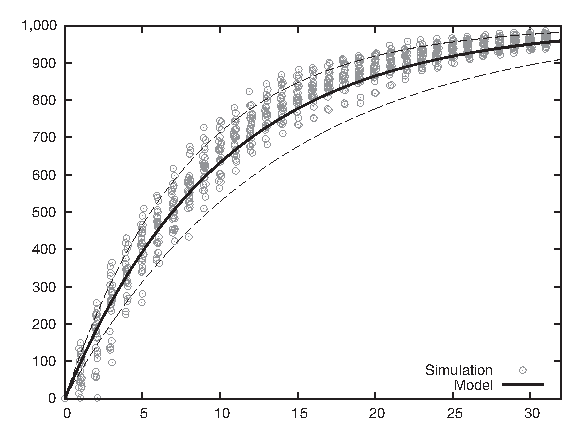
\includegraphics{img/visitssimul}}
  \caption{Unique visitors as a function of time: results from the
    simulation run, together with predictions from the analytical
    model. All data points are jittered horizontally to minimize
    overplotting. The solid line is the most probable number of
    visitors according to the model; the dashed lines indicate a
    confidence band.}
  \label{fig:visitorssimul}
\end{figure}

Figure \ref{fig:visitorssimul} also includes results from the
analytical model. In Chapter \ref{ch:probability}, we found that the
number of unique visitors on day $t$ was given by:
%
\[
n(t) = N \paren{ 1 - e^{-\frac{k}{N} t}} 
\]
%
where $N$ is the total number of visitors ($N = \text{1,000}$ in the
simulation) and $k$ is the average number of visitors per day ($k =
100$ in the simulation). Accordingly, the solid line in Figure
\ref{fig:visitorssimul} is given by $n(t) = \text{1,000} \paren{ 1 -
  \exp \paren{-\frac{100}{1000} t} }$.

The simulation includes a parameter that was not part of the
analytical model---namely the width $s$ of the daily fluctuations in
visitors. I have chosen the value $s = 50$ for the simulation runs.
The dashed lines in Figure \ref{fig:visitorssimul} show the analytical
model, with values of $k \pm s/2$ (\ie, $k=75$ and $k=125$) to provide
a sense for the predicted spread, according to the mean-field model.

First of all, we should note that the analytical model agrees very
well with the data from the simulation run: that's a nice confirmation\vadjust{\pagebreak}
of our previous result! But we should also note the differences; in
particular, the simulation results are consistently \emph{higher} than
the theoretical predictions. If we think about this for a moment, this
makes sense. If on any day there are unusually many visitors, then
this irrevocably bumps the number of unique visitors \emph{up}: the
number of unique visitors can never shrink, so any outlier above the
average can never be neutralized (in contrast to an outlier below the
average, which can be compensated by any subsequent high-traffic day).

We can further analyze the data from the simulation run, depending on
our needs. For instance, we can calculate the most probable value for
each day, and we can estimate proper confidence intervals around it.
(We will need more than 25 trials to obtain a good estimate of the
latter.)

What is more interesting about the simulation model developed here is
that we can use it to obtain \emph{additional} information that would
be difficult or impossible to calculate from the analytical formula.
For example, we may ask for the \emph{distribution of visits per user}
(\ie, how many users have visited once, twice, three times, and so
on). The answer to this question is just a snap of the fingers away!
We can also extend the model and ask for the number of unique visitors
who have paid \emph{two or more} visits (not just one). (For two
visits per person, this question can be answered within the framework
of the original analytical model, but the calculations rapidly become
more tedious as we are asking for higher visit counts per person.)

Finally, we can extend the simulation to include features not included
in the analytical model at all. For instance, for a real website, not
all possible visitors are equally likely to visit: some individuals
will have a higher probability of visiting the website than do others.
It would be very difficult to incorporate this kind of generalization
into the approach taken in Chapter \ref{ch:probability}, because it
contradicts the basic assumption that the fraction of actual repeat
visitors equals the fraction of repeat visitors in the total
population. But it is not at all difficult to model this behavior in a
simulation model!

\index{Monte Carlo simulations!outcome distributions|)}
\index{distributions!Monte Carlo simulation outcome distributions|)}

% \subsection{Optional: Monte-Carlo Simulation as Integration}
% 
% shooting for pi
% shooting for pretzels
% bayesian likelihood fct evaluation (?)

\subsection{Pro and Con}

\index{Monte Carlo simulations!issues}
 
Basic simulations of the kind discussed in this section are often easy
to program---certainly as compared with the effort required to develop
nontrivial combinatorial arguments! Moreover, when we start writing a
simulation project, we can be fairly certain of being successful in
the end; whereas there is no guarantee that an attempt to find an
exact answer to a combinatorial problem will lead anywhere.

On the other hand, we should not forget that a simulation produces
numbers, not insight! A simulation is always only one step in a larger
process, which must include a proper analysis of the results from the
simulation run and, ideally, also involves an attempt to incorporate
the simulation data into a larger conceptual model. I always get a
little uncomfortable when presented with a bunch of simulation results
that have not been fit into a larger context.  Simulations cannot
replace analytical modeling.

In particular, simulations do not yield the kind of insight into the
mechanisms driving certain developments that a good analytical model
affords. For instance, recall the case study near the end of Chapter
\ref{ch:scaling}, in which we tried to determine the optimal number of
servers. One important insight from that model was that the
probability $p^n$ for a total failure dropped extremely rapidly as the
number $n$ of servers increased: the exponential decay (with $n$) is
much more important than the reliability $p$ of each individual
server. (In other words, redundant commodity hardware beats expensive
supercomputers---at least for situations in which this simplified cost
model holds!) This is the kind of insight that would be difficult to
gain simply by looking at results from simulation runs.

Simulations can be valuable for verifying analytical work and for
extending it by incorporating details that would be difficult or
impossible to treat in an analytical model. At the same time, the
benefit that we can derive from simulations is enhanced by the insight
gained from the analytical, conceptual modeling of the the mechanisms
driving a system.

The two methods are complementary---although I will give primacy to
analytical work. Analytical models without simulation may be crude
but will still yield insight, whereas simulations without analysis
produce only numbers, not insight.

\index{simulations!Monte Carlo simulations|)}
\index{Monte Carlo simulations|)}

% ============================================================
\section{Resampling Methods}

\index{simulations!resampling methods|(} 
\index{resampling methods, simulations|(}
 
Imagine you have taken a sample of $n$ points from some population.
It is now a trivial exercise to calculate the mean from this sample.
But how reliable is this mean? If we repeatedly took new samples (of
the same size) from the population and calculated \emph{their}
means, how much would the various values for the mean jump around?

This question is important. A point estimate (such as the mean by
itself) is not very powerful: what we really want is an interval
estimate which also gives us a sense of the reliability of the
answer.

If we could go back and draw additional samples, then we could obtain
the distribution of the mean directly as a histogram of the observed
means. But that is not an option: all we have are the $n$ data points
of the original sample.

Much of classical statistics deals with precisely this question: how
can we make statements about the reliability of an estimate based
only on a set of observations? To make progress, we need to make some
assumptions about the way values are distributed. This is where the
\emph{sampling distributions} of classical statistics come in: all
those Normal, $t$, and chi-square distributions (see Chapter
\ref{ch:statistics}). Once we have a theoretical model for the way
points are distributed, we can use this model to establish confidence
intervals.

Being able to make such statements is one of the outstanding
achievements of classical statistics, but at the same time, the
difficulties in getting there are a major factor in making classical
statistics seem so obscure. Two problems stand out:

\begin{itemize}
\item Our assumptions about the shape of those distributions may not
  be correct, or we may not be able to formulate those distributions
  at all---in particular, if we are interested in more complicated
  quantities than just the sample mean or if we are dealing with
  populations that are ill behaved (\ie, not even remotely Gaussian).
\item Even if we know the sampling distribution, determining
  confidence limits from it may be tedious, opaque, and error-prone.
\end{itemize}

\subsection{The Bootstrap}

\index{bootstrap|(}
\index{confidence intervals!bootstrap}  

The \emph{bootstrap} is an alternative approach for finding confidence
intervals and similar quantities directly from the data. Instead of
making assumptions about the distribution of values and then employing
theoretical arguments, the bootstrap goes back to the original idea:
what if we could draw \emph{additional samples} from the population?

We can't go back to the original population, but the sample that we
already have should be a fairly good approximation to the overall
population. We can therefore create additional samples (also of size
$n$) by \emph{sampling with replacement} from the original sample.
For each of these ``synthetic'' samples, we can calculate the mean (or
any other quantity, of course) and then use this set of values for the
mean to determine a measure of the spread of its distribution via any
standard method (\eg, we might calculate its inter-quartile range; see
Chapter \ref{ch:univariate}).

Let's look at an example---one that is simple enough that we can work
out the analytical answer and compare it directly to the bootstrap
results. We draw $n = 25$ points from a standard Gaussian distribution
(with mean $\mu = 0$ and standard deviation $\sigma = 1$). We then ask
about the (observed) sample mean and more importantly, about its
standard error. In this case, the answer is simple: we know that the
error of the mean is $\sigma/\sqrt{n}$ (see Chapter \ref{ch:bigfoot}),
which amounts to $1/5$ here. This is the analytical result.

To find the bootstrap estimate for the standard error, \index{standard error!bootstrap estimate} we draw $100$
samples, each containing $n = 25$ points, from our original sample of
$25$ points. Points are drawn randomly with replacement (so that each
point can be selected multiple times). For each of these bootstrap
samples, we calculate the mean. Now we ask: what is the spread of the
distribution of these 100 bootstrap means?

The data is plotted in Figure \ref{fig:bootstrap}. At the bottom, we
see the $25$ points of the original data sample; above that, we see
the means calculated from the $100$ bootstrap samples. (All points are
jittered vertically to minimize overplotting.) In addition, the figure
shows 
kernel density estimates (see Chapter \ref{ch:univariate}) of the
original sample and also of the bootstrap means. The latter is the
answer to our original question: if we repeatedly took samples from
the \emph{original} distribution, the sample means would be distributed
similarly to the bootstrap means.

\begin{figure}
  \centerline{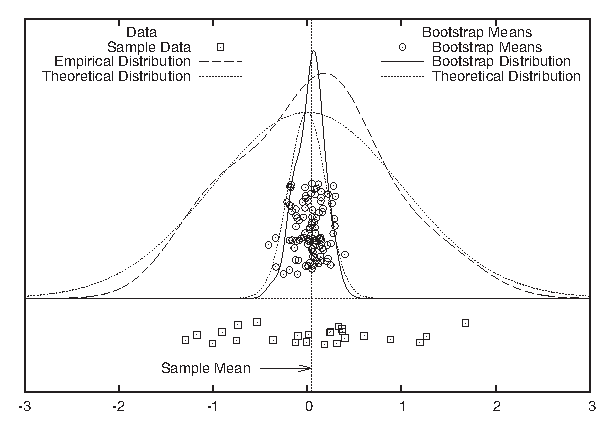
\includegraphics{img/bootstrap}}
  \caption{The bootstrap. The points in the original sample are shown
    at the bottom; the means calculated from the bootstrap samples are
    shown above. Also displayed are the original distribution and the
    distribution of the sample means, both using the theoretical result
    and a kernel density estimate from the corresponding samples.}
  \label{fig:bootstrap}\vspace*{-6pt}
\end{figure}

(Because in this case we happen to know the original distribution, we
can also plot both it and the theoretical distribution of the mean,\vadjust{\pagebreak}
which happens to be Gaussian as well but with a reduced standard
deviation of $\sigma/\sqrt{n}$. As we would expect, the theoretical
distributions agree reasonably well with the kernel density estimated
calculated from the data.)

Of course, in this example the bootstrap procedure was not necessary.
It should be clear, however, that the bootstrap provides a simple
method for obtaining confidence intervals even in situations where
theoretical results are not available. For instance, if the original
distribution had been highly skewed, then the Gaussian assumption
would have been violated.  Similarly, if we had wanted to calculate a
more complicated quantity than the mean, analytical results might have
been hard to obtain.

Let me repeat this, because it's important: bootstrapping is a method
to estimate the \emph{spread} of some quantity. It is not a method to
obtain ``better'' estimates of the original quantity itself---for
that, it is necessary to obtain a larger sample by making additional
drawings from the original population.  The bootstrap is not a way to
give the appearance of a larger sample size by reusing points!

\vspace*{-6pt}
\subsection{When Does Bootstrapping Work?}

As we have seen, the bootstrap is a simple, practical, and relatively
transparent method to obtain confidence intervals for estimated
quantities. This begs the question: when does it work?  The following
two conditions must be fulfilled.
\begin{enumerate}
\item The original sample must provide a good representation of the
  entire population.
\item The estimated quantity must depend ``smoothly'' on the data
  points.
\end{enumerate}

The first condition requires the original sample to be sufficiently
large and relatively clean. If the sample size is too small, then the
original estimate for the actual quantity in question (the mean, in
our example) won't be very good. (Bootstrapping in a way exacerbates
this problem because data points have a greater chance of being reused
repeatedly in the bootstrap samples.) In other words, the original
sample has to be large enough to allow meaningful estimation of the
primary quantity. Use common sense and insight into your specific
application area to establish the required sample size for your
situation.

Additionally, the sample has to be relatively clean: crazy outliers,
for instance, can be a problem. Unless the sample size is very large,
outliers have a significant chance of being reused in a bootstrap
sample, distorting the results.

Another problem exists in situations involving power-law
distributions. As we saw in Chapter \ref{ch:probability}, estimated
values for such distributions may not be unique but depend on the
sample \emph{size}. Of course, the same considerations apply to
bootstrap samples drawn from such distributions.

The second condition suggests that bootstrapping does not work well
for quantities that depend critically on only a few data points. For
example, we may want to estimate the maximum value of some
distribution.  Such an estimate depends critically on the largest
observed value---that is, on a single data point. For such
applications, the bootstrap is not suitable. (In contrast, the mean
depends on \emph{all} data points and with equal weight.)

Another questions concerns the number of bootstrap samples to take.
The short answer is: as many as you need to obtain a sufficiently good
estimate for the spread you are calculating. If the number of points
in the original sample is very small, then creating too many bootstrap
samples is counterproductive because you will be regenerating the same
bootstrap samples over and over again. However, for reasonably sized
samples, this is not much of a problem, since the number of possible
bootstrap samples grows very quickly with the number of data points
$n$ in the original sample.  Therefore, it is highly unlikely that the
same bootstrap example is generated more than once---even if we
generate thousands of bootstrap samples.

The following argument will help to develop a sense for the order of
magnitudes involved.  The problem of choosing $n$ data points with
replacement from the original $n$-point sample is equivalent to
assigning $n$ elements to $n$ cells. It is a classical problem in
occupancy theory to show that there are:
%
\[
\binom{2n - 1}{n} = \frac{(2n - 1)!}{n! (n-1)!}
\]
%
ways of doing this. This number grows extremely quickly: for $n=5$ it
is $126$, for $n=10$ we have 92,378, but for $n=20$ it already exceeds
$10^{10}$.

(The usual proof proceeds by observing that assigning $r$
indistinguishable objects to $n$ bins is equivalent to aligning $r$
objects and $n-1$ bin dividers.\vadjust{\pagebreak}  There are $r+n-1$ spots in total,
which can be occupied by either an object or a divider, and the
assignment amounts to choosing $r$ of these spots for the $r$ objects.
The number of ways one can choose $r$ elements out of $n+r-1$ is given
by the binomial coefficient $\binom{r+n-1}{r}$. Since in our case $r =
n$, we find that the number of different bootstrap samples is given by
the expression above.)

\vspace*{-6pt}
\subsection{Bootstrap Variants}

There are a few variants of the basic bootstrap idea. The method so
far---in which points are drawn directly from the original sample---is
known as the \emph{nonparametric bootstrap}. \index{nonparametric bootstrap} An alternative is
the
\emph{parametric bootstrap}: \index{parametric bootstrap} in this case, we assume that the original
population follows some particular probability distribution (such as
the Gaussian), and we estimate its parameters (mean and standard
deviation, in this case) from the original sample. The bootstrap
samples are then drawn from this distribution rather than from the
original sample. The advantage of the parametric bootstrap is that the
bootstrap values do not have to coincide exactly with the known data
points. In a similar spirit, we may use the original sample to compute
a kernel density estimate (as an approximation to the population
distribution) and then draw bootstrap samples from it. This method
combines aspects of both parametric and nonparametric approaches: it
is nonparametric (because it make no assumption about the form of the
underlying population distribution), yet the bootstrap samples are not
restricted to the values occurring in the original sample. In
practice, neither of these variants seems to provide much of an
advantage over the original idea (in part because the number of
possible bootstrap samples grows so quickly with the number of points
in the sample that choosing the bootstrap samples from only those
points is not much of a restriction).

Another idea (which historically predates the bootstrap) is the
so-called \emph{jackknife}. \index{jackknife} In the jackknife, we don't draw random
samples. Instead, given an original sample consisting of $n$ data
points, we calculate the $n$ estimates of the quantity of interest by
successively omitting one of the data points from the sample. We can
now use these $n$ values in a similar way that we used values
calculated from bootstrap samples. Since the jackknife does not
contain any random element, it is an entirely deterministic procedure.

\index{bootstrap|)}
\index{simulations!resampling methods|)} 
\index{resampling methods, simulations|)}

\vspace*{-6pt}
% ============================================================
\section{Workshop: Discrete Event Simulations with SimPy}

\index{simulations!discrete event simulations with SimPy|(}
\index{SimPy|(}
  
All the simulation examples that we considered so far were either
static (coin tosses, Monty Hall problem) or extremely stripped down
and conceptual (unique visitors).  But if we are dealing with the
behavior and time development of more complex systems---\break consisting of
many different particles or actors that interact with each other in
complicated ways---then we want a simulation that expresses all these
entities in a manner that closely resembles the problem domain. In
fact, this is probably exactly what most of us think of when we hear
the term ``simulation.''

There are basically two different ways that we can set up such a
simulation. In a \emph{continuous time simulation}, \index{continuous time simulations} time progresses in
``infinitesimally''\vadjust{\pagebreak} small increments. At each time step, all
simulation objects are advanced while taking possible interactions or
status changes into account. We would typically choose such an
approach to simulate the behavior of particles moving in a fluid or a
similar system.

But in other cases, this model seems wasteful. For instance, consider
customers arriving at a bank: in such a situation, we only care about
the \emph{events} that change the state of the system (\eg, customer
arrives, customer leaves)---we don't actually care what the customers
do while waiting in line! For such system we can use a different
simulation method, known as \emph{discrete event simulation}. \index{discrete event simulations} In this
type of simulation, time does not pass continuously; instead, we
determine when the next event is scheduled to occur and then jump
ahead to exactly that moment in time.

\enlargethispage{6pt}

Discrete event simulations are applicable to a wide variety of
problems involving multiple users competing for access to a shared
server.  It will often be convenient to phrase the description in
terms of the proverbial ``customers arriving at a bank,'' but exactly
the same considerations apply, for instance, to messages on a computer
network.


\vspace*{-6pt}
\subsection{Introducing SimPy}

\index{SimPy!about|(}
 
The SimPy package (\url{http://simpy.sourceforge.net/}) is a Python project to build discrete
event simulation models. The framework handles all the event scheduling and
messaging ``under the covers'' so that the programmer can concentrate
on describing the behavior of~the actors in the simulation.

All actors in a SimPy simulation must be subclasses of the class
\texttt{Process}. Congestion points where queues form are modeled by
instances of the \texttt{Resource} class or its subclasses.  Here is a
short example, which describes a customer visiting a bank:

\begin{verbatim}
from SimPy.Simulation import *

class Customer( Process ):
    def doit( self ):
        print "Arriving"
        yield request, self, bank

        print "Being served"
        yield hold, self, 100.0

        print "Leaving"
        yield release, self, bank


# Beginning of main simulation program
initialize()

bank = Resource()

cust = Customer()
cust.start( cust.doit() )

simulate( until=1000 )
\end{verbatim}

Let's skip the class definition of the \texttt{Customer} object for
now and concentrate on the rest of the program. The first function to
call in any SimPy program is the \texttt{initialize()} method, which
sets up the simulation run and sets the ``simulation clock'' to zero.
We then proceed to create a \texttt{Resource} object (which models the
bank) and a single \texttt{Customer} object. After creating the
\texttt{Customer}, we need to activate it via the \texttt{start()}
member function. \index{start() function} The \texttt{start()} function takes as argument the
function that will be called to advance the \texttt{Customer} through
its life cycle (we'll come back to that).  Finally, we kick off the
actual simulation, requiring it to stop after 1,000 time steps on the
simulation clock have passed.

The \texttt{Customer} subclasses \texttt{Process}, therefore its
instances are active agents, which will be scheduled by the framework
to receive events. Each agent must define a \emph{process execution
  method} (PEM),\index{PEM (process execution method)}\index{process
execution method (PEM)} which defines its behavior and which will be invoked by
the framework whenever an event occurs.

For the \texttt{Customer} class, the PEM is the \texttt{doit()}
function. (There are no restrictions on its name---it can be called
anything.)  The PEM describes the customer's behavior: after the
customer arrives, the customer \emph{requests} a resource instance
(the \texttt{bank} in this case). If the resource is not available
(because it is busy, serving other customers), then the framework will
add the customer to the waiting list (the \emph{queue}) for the
requested resource. Once the resource becomes available, the customer
is being serviced. In this simple example, the service time is a fixed
value of 100 time units, during which the customer instance is
\emph{holding}---just waiting until the time has passed. When service
is complete, the customer \emph{releases} the resource instance. Since
no additional actions are listed in the PEM, the customer is not
scheduled for future events and will disappear from the simulation.

Notice that the \texttt{Customer} interacts with the simulation
environment through Python \texttt{yield} statements, using special
yield expressions of the form shown in the example.  Yielding control
back to the framework in this way ensures that the \texttt{Customer}
retains its state and its current spot in the life cycle between
invocations.  Although there are no restrictions on the name and
argument list permissible for a PEM, each PEM \emph{must} contain at
least one of these special \texttt{yield} statements. (But of course
not necessarily all three, as in this case; we are free to define the
behavior of the agents in our simulations at will.)

% XXX --- XXX    should doit() be called go() ?

\index{SimPy!about|)}

\subsection{The Simplest Queueing Process}

\index{SimPy!queueing|(}
\index{queueing, SimPy!|(}  

Of course the previous example which involved only a \emph{single}
customer entering and leaving the bank, is not very exciting---we
hardly needed a simulation for that! Things change when we have more
than one customer in the system at the same time.

The listing that follows is very similar to the previous example,
except that now there is an infinite stream of customers arriving at
the bank and requesting service. To generate this infinite sequence of
customers, the listing makes use of an idiom that's often used in
SimPy programs: a ``source'' (the \texttt{CustomerGenerator}
instance).

\begin{verbatim}
from SimPy.Simulation import *
import random as rnd

interarrival_time = 10.0
service_time = 8.0


class CustomerGenerator( Process ):
    def produce( self, b ):
        while True:
            c = Customer( b )
            c.start( c.doit() )
            yield hold, self, rnd.expovariate(1.0/interarrival_time)


class Customer( Process ):
    def __init__( self, resource ):
        Process.__init__( self )
        self.bank = resource
    
    def doit( self ):
        yield request, self, self.bank
        yield hold, self, self.bank.servicetime()
        yield release, self, self.bank

class Bank( Resource ):
    def servicetime( self ):
        return rnd.expovariate(1.0/service_time)


initialize()

bank = Bank( capacity=1, monitored=True, monitorType=Monitor )

src = CustomerGenerator()
activate( src, src.produce( bank ) )

simulate( until=500 )
\end{verbatim}
\begin{verbatim}

print bank.waitMon.mean()
print

for evt in bank.waitMon:
    print evt[0], evt[1]
\end{verbatim}\vspace*{-4pt}

The \texttt{CustomerGenerator} is itself a subclass of
\texttt{Process} and defines a PEM (\texttt{produce()}). Whenever it
is triggered, it generates a new \texttt{Customer} and then goes back
to sleep for a random amount of time. (The time is distributed
according to an exponential distribution---we will discuss this
particular choice in a moment.) Notice that we don't need to keep
track of the \texttt{Customer} instances explicitly: once they have
been activated using the \texttt{start()} member function, the
framework ensures that they will receive scheduled events.

There are two changes to the \texttt{Customer} class. First of all, we
explicitly inject the resource to request (the \texttt{bank}) as an
additional argument to the constructor. By contrast, the
\texttt{Customer} in the previous example found the \texttt{bank}
reference via lookup in the global namespace. That's fine for small
programs but becomes problematic for larger ones---especially if
there is more than one resource that may be requested. The second
change is that the \texttt{Customer} now asks the \emph{bank} for the
service time. This is in the spirit of problem domain modeling---it's
usually the server (in this case, the bank) that controls the time it
takes to complete a transaction.  Accordingly, we have introduced
\texttt{Bank} as subclass of \texttt{Resource} in order to accommodate
this additional functionality. (The service time is also exponentially
distributed but with a different wait time than that used for the
\texttt{CustomerGenerator}.)

Subtypes of the \texttt{Process} class \index{Process class} are used to model actors in a
SimPy simulation. Besides these active simulation objects, the next
most important abstraction describes congestion points, modeled by the
\texttt{Resource} class \index{Resource class} and its subclasses. Each \texttt{Resource}
instance models a shared resource that actors may request, but its
more important function is to manage the \emph{queue} of actors
currently waiting for access.

Each \texttt{Resource} instance consists of a single queue and one or
more actual ``server units'' that can fulfill client requests. Think
of the typical queueing discipline followed in banks and post offices
(in the U.S.---other countries have different conventions!): a single
line but multiple teller windows, with the person at the head of the
line moving to the next available window. That is the model
represented by each \texttt{Resource} instance. The number of server
units is controlled through the keyword argument \texttt{capacity} to
the \texttt{Resource} constructor. Note that all server units in a
single \texttt{Resource} instance are identical. Server units are also
``passive'': they have no behavior themselves. They only exist so that
a \texttt{Process} object can acquire them, hold them for a period of
time, and then release them (like a mutex).

Although a \texttt{Resource} instance may have multiple server units,
it can contain only a single queue. If you want to model a supermarket
checkout situation, where each server unit has its own queue, you
therefore need to set up multiple \texttt{Resource} instances, each
with \texttt{capacity=1}: one for each checkout stand and each
managing its own queue of customers. 

For each \texttt{Resource} instance, we can monitor \index{Monitor class} the length of the
queue and the events that change it (arrivals and departures) by
registering an observer object with the \texttt{Resource}. There are
two types of such observers in SimPy: a \texttt{Monitor} records the
time stamp and new queue length for every event that affects the
queue, whereas a \texttt{Tally} \index{Tally class} only keeps enough information to
calculate summary information (such as the average queue length).  Here
we have registered a \texttt{Monitor} object with the \texttt{Bank}.
(We'll later see an example of a \texttt{Tally}.)

\begin{figure}
  \centerline{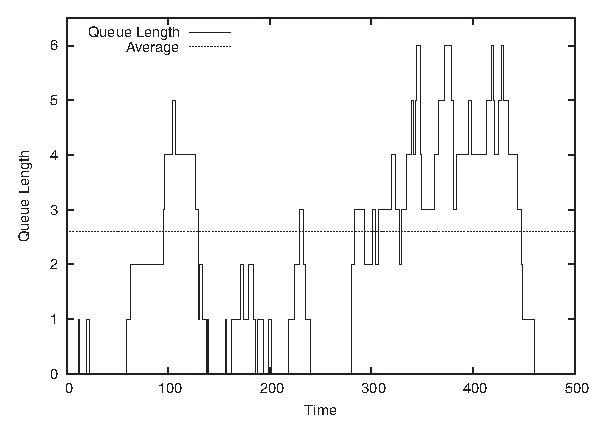
\includegraphics{img/simpy2}}
  \caption{Number of customers in queue over time.}\label{fig:simpy2}\vspace*{-6pt}
\end{figure}

As before, we run the simulation until the internal simulation clock
reaches 1,000.  The \texttt{CustomerGenerator} produces an infinite
stream of \texttt{Customer} objects, each requesting service from the
\texttt{Bank}, while the \texttt{Monitor} records all changes to the
queue.

After the simulation has run to completion, we retrieve the
\texttt{Monitor} object from the \texttt{Bank}: if an observer had
been registered with a \texttt{Resource}, then it is available in the
\texttt{waitMon} member variable.  We print out the average queue
length over the course of the simulation as well as the full time
series of events. (The \texttt{Monitor} class is a \texttt{List}
subclass, so we can iterate over it directly.) The time evolution of
the queue is shown in Figure \ref{fig:simpy2}.

One last implementation detail: if you look closely, you will notice
that the \texttt{CustomerGenerator} is activated using the standalone
function \texttt{activate()}. \index{activate() function} This function is an alternative to the
\texttt{start()} member function of all \texttt{Process} objects and
is entirely equivalent to it.

\vspace*{-6pt}
\subsection{Optional: Queueing Theory}

Now that we have seen some of these concepts in action already, it
is a good time to step back and fill in some theory.

A queue is a specific example of a \emph{stochastic process}. \index{stochastic processes} In
general, the term ``stochastic process'' refers to a sequence of
random events occurring in time. In the queueing example, customers
are joining or leaving the queue at random times, which makes the queue
grow and shrink accordingly. Other examples of stochastic processes
include random walks, the movement of stock prices, and the inventory
levels in a store.  (In the latter case, purchases by customers and
possibly even deliveries by suppliers constitute the random events.)

In a queueing problem, we are concerned only about arrivals and
departures.  A particularly important special case
 assumes that the rate at
which customers arrive is constant over time and that arrivals at
different times are independent of each other. (Notice that these are
reasonable assumptions in many cases.)  These two conditions imply
that the number of arrivals during a certain time period $t$ follows a
Poisson distribution, since the Poisson distribution:
%
\[
p(k, t, \lambda) = \frac{(\lambda t)^k}{k!} e^{-\lambda t}
\]
%
gives the probability of observing $k$ Successes (arrivals, in our
case) during an interval of length $t$ if the ``rate'' of Successes is
$\lambda$ (see Chapter \ref{ch:probability}).

Another consequence is that the times between arrivals are distributed
according to an exponential distribution:
%
\[
 p(t, \lambda) = \lambda e^{-\lambda t}
\]
%
The mean of the exponential distribution\index{exponential
distribution}\index{mean!exponential distribution} can be calculated without
difficulty and equals $1/\lambda$.  It will often be useful to work with its
inverse $t_a = 1/\lambda$, the \emph{average interarrival
  time}.

(It's not hard to show that interarrival times are distributed
according to the exponential distribution when the number of arrivals
per time interval follows a Poisson distribution. Assume that an
arrival occurred at $t=0$.  Now we ask for the probability that
\emph{no} arrival has occurred by $t=T$; in other words, $p(0, T,
\lambda) = e^{-\lambda T}$ because $x^0 = 1$ and $0! = 1$.
Conversely, the probability that the next arrival will have occurred
sometime between $t=0$ and $t=T$ is $1 - p(0,T,\lambda)$. This is the
cumulative distribution function for the interarrival time, and from
it, we find the probability density for an arrival to occur at $t$ as
$\frac{\rm d}{{\rm d}t}%\Diff{\displaystyle t}
 \paren{ 1 - p(0,t,\lambda) } = \lambda e^{-\lambda t}$.)

The appearance of the exponential distribution as the distribution of
interarrival times deserves some comment. At first glance, it may seem
surprising because this distribution is greatest for small
interarrival times, seemingly favoring very short intervals. However,
this observation has to be balanced against the infinity of possible
interarrival times, all of which may occur! What is more important is
that the exponential distribution is in a sense the most ``random''
way that interarrival times can be distributed: no matter how long we
have waited since the last arrival, the probability that the next
visitor will arrive after $t$ more minutes is always \emph{the same}:
$p(t, \lambda) = \lambda e^{-\lambda t}$. This property is often
referred to as the \emph{lack of memory} of the exponential
distribution. Contrast this with a distribution of interarrival times
that has a peak for some nonzero time: such a distribution describes a
situation of \emph{scheduled} arrivals, as we would expect to occur at
a bus stop. In this scenario, the probability for an arrival to occur
within the next $t$ minutes will change with time.

Because the exponential distribution arises naturally from the
assumption of a constant arrival rate (and from the independence of
different arrivals), we have used it as the distribution of
interarrival times in the \texttt{CustomerGenerator} in the previous
example. It is less of a natural choice for the distribution of
service times (but it makes some theoretical arguments simpler).

The central question in all queueing problems concerns the expected
length of the queue---not only how large it is but also whether it
will settle down to a finite value at all, or whether it will
``explode,'' growing beyond all bounds.

In the simple memoryless, single-server--single-queue scenario that we
have been investigating, the only two control parameters are the
arrival rate $\lambda_a$ and the service or exit rate $\lambda_e$; or
rather their ratio:
%
\[
u = \frac{\lambda_a}{\lambda_e}
\]
%
which is the fraction of time the server is busy. The quantity $u$ is
the server's \emph{utilization}.  It is intuitively clear that if the
arrival rate is greater than the exit rate (\ie, if customers are
arriving at a faster rate then the server can process them), then the
queue length will explode. However, it turns out that even if the
arrival rate \emph{equals} the service rate (so that $u = 1$), the
queue length still grows beyond all bounds. Only if the arrival rate
is strictly lower than the service rate will we end up with a finite
queue.

Let's see how this surprising result can be derived. Let $p_n$ be the
probability of finding exactly $n$ customers waiting in the queue.
The rate at which the queue grows is $\lambda_a$, but the rate at
which the queue grows from exactly $n$ to exactly $n+1$ is $\lambda_a
p_n$, since we must take into account the probability of the queue
having exactly $n$ members. Similarly, the probability of the queue
shrinking from $n+1$ to $n$ members is $\lambda_e p_{n+1}$.

In the steady state (which is the requirement for a finite queue
length), these two rates must be equal:
%
\[
\lambda_a p_n = \lambda_e p_{n+1}
\]
%
which we can rewrite as:
%
\[
p_{n+1} = \frac{\lambda_a}{\lambda_e} p_n = u p_n
\]
%
This relationship must hold for all $n$, and therefore we can repeat
this argument and write $p_n = u p_{n-1}$ and so on. This leads to an
expression for $p_n$ in terms of $p_0$:
%
\[
p_n = u^n p_0
\]
%
The probability $p_0$ is the probability of finding \emph{no} customer
in the queue---in other words, it is the probability that the server
is idle. Since the utilization is the probability for the server to be
busy, the probability $p_0$ for the server to be idle must be $p_0 =
1-u$.

We can now ask about the expected length $L$ of the queue. We already
know that the queue has length $n$ with probability $p_n = u^n p_0$.
Finding\vadjust{\pagebreak} the expected queue length $L$ requires that we sum over all
possible queue lengths, each one weighted by the appropriate
probability:\vspace*{-2pt}
%
\begin{align*}
L & = \sum_{n=0}^\infty n p_n \\
  & = p_0 \sum_{n=0}^\infty n u^n
\end{align*}
%\Diff{\displaystyle u}
Now we employ a trick that is often useful for sums of this form: 
observe that $\frac{\rm d}{{\rm d}u} u^n = n u^{n-1}$ and
hence that $n u^n = u
\frac{\rm d}{{\rm d}u} u^n$. Using this expression in the sum for $L$ leads
to:\vspace*{-2pt}
%
\begin{align*}
L & = p_0 \sum_{n=0}^\infty u \Diff{u} u^n \\
  & = p_0 u \Diff{u} \sum_{n=0}^\infty u^n \\
  & = p_0 u \Diff{u} \frac{1}{1-u} \qquad \text{(geometric series)} \\
  & = p_0 \frac{u}{(1-u)^2} \\
  & = \frac{u}{1-u}
\end{align*}
%
where we have used the sum of the geometric series (see Appendix
\ref{app:calculus}) and the expression for $p_0 = 1-u$. We can rewrite
this expression directly in terms of the arrival and exit rates
as:\vspace*{-2pt}
%
\[ 
L = \frac{u}{1-u} = \frac{\lambda_a}{\lambda_e - \lambda_a}
\]
%

This is a central result. It gives us the expected length of the queue
in terms of the utilization (or in terms of the arrival and exit
rates). For low utilization (\ie, an arrival rate that is much lower
than the service rate or, equivalently, an interarrival time that is
much larger than the service time), the queue is very short on
average.  (In fact, whenever the server is idle, then the queue length
equals $0$, which drags down the average queue length.)  But as the
arrival rate approaches the service rate, the queue grows in length
and becomes infinite when the arrival rate equals the service rate.
(An intuitive argument for why the queue length will explode when the
arrival rate equals the service time is that, in this case, the server
never has the opportunity to ``catch up.'' If the queue becomes longer
due to a chance fluctuation in arrivals, then this backlog will
persist forever, since overall the server is only capable of keeping
up with arrivals. The cumulative effect of such chance fluctuations
will eventually make the queue length diverge.)

% Although we have derived it under the assumption that the system
% is memoryless (...)

% Obviously, we have only scratched the surface of queueing theory. 
% FIFO;  (balking, reneging, jockeying)

\index{SimPy!queueing|)}
\index{queueing|SimPy!|)}  

\subsection{Running SimPy Simulations}

\index{SimPy!running simulations|(}
 
In this section, we will try to confirm the previous result regarding
the expected queue length by simulation. In the process, we will
discuss a few practical points of using SimPy to understand queueing
systems.

First of all, we must realize that each simulation run is only a
particular realization of the sequence of events. To draw conclusions
about the system in general, we therefore always need to perform
several simulation runs and average their results.

In the previous listing, the simulation framework maintained its state
in the global environment. Hence, in order to rerun the simulation,
you had to restart the entire program! The program in the next listing
uses an alternative interface that encapsulates the entire environment
for each simulation run in an instance of class \texttt{Simulation}. \index{Simulation class} 
The global functions \texttt{initialize()}, \texttt{activate()}, and
\texttt{simulate()} are now member functions of this
\texttt{Simulation} object. Each instance of the \texttt{Simulation}
class provides a separate, isolated simulation environment. A
completely new simulation run now requires only that we create a new
instance of this class.

The \texttt{Simulation} class is provided by SimPy. Using it does not
require any changes to the previous program, except that the current
instance of the \texttt{Simulation} class must be passed explicitly to
all simulation objects (\ie, instances of \texttt{Process} and
\texttt{Resource} and their subclasses):

\begin{verbatim}
from SimPy.Simulation import *
import random as rnd

interarrival_time = 10.0

class CustomerGenerator( Process ):
    def produce( self, bank ):
        while True:
            c = Customer( bank, sim=self.sim )
            c.start( c.doit() )
            yield hold, self, rnd.expovariate(1.0/interarrival_time)


class Customer( Process ):
    def __init__( self, resource, sim=None ):
        Process.__init__( self, sim=sim )
        self.bank = resource
    
    def doit( self ):
        yield request, self, self.bank
        yield hold, self, self.bank.servicetime()
        yield release, self, self.bank

class Bank( Resource ):
    def setServicetime( self, s ):
        self.service_time = s
        
    def servicetime( self ):
        return rnd.expovariate(1.0/self.service_time )


def run_simulation( t, steps, runs ):
    for r in range( runs ):
\end{verbatim}
\begin{verbatim}
        sim = Simulation()
        sim.initialize()
        
        bank = Bank( monitored=True, monitorType=Tally, sim=sim )
        bank.setServicetime( t )

        src = CustomerGenerator( sim=sim )
        sim.activate( src, src.produce( bank ) )

        sim.startCollection( when=steps//2 )
        sim.simulate( until=steps )
        
        print t, bank.waitMon.mean()
    

t = 0
while t <= 11.0:
    t += 0.5
    run_simulation( t, 100000, 10 )
\end{verbatim}

Another important change is that we don't start recording until half
of the simulation time steps have passed (that's what the
\texttt{startCollection()} method is for). Remember that we are
interested in the queue length in the \emph{steady state}---for that
reason, we don't want to start recording until the system has settled
down and any transient behavior has disappeared.

To record the queue length, we now use a \texttt{Tally} object \index{Tally class} instead
of a \texttt{Monitor}. The \texttt{Tally} will not allow us to replay
the entire sequence of events, but since we are only interested in the
average queue length, it is sufficient for our current purposes.

Finally, remember that as the utilization approaches $u=1$ (\ie, as
the service time approaches the interarrival time), we expect the queue
length to become infinite. Of course, in any finite simulation it is
impossible for the queue to grow to infinite length: the length of the
queue is limited by the finite duration of the simulation run.  The
consequence of this observation is that, for utilizations near or
above $1$, the queue length that we will observe depends on the number
of steps that we allow in the simulation. If we terminate the
simulation too quickly, then the system will not have had time to
truly reach its fully developed steady state and so our results will
be misleading.


\begin{figure}
  \centerline{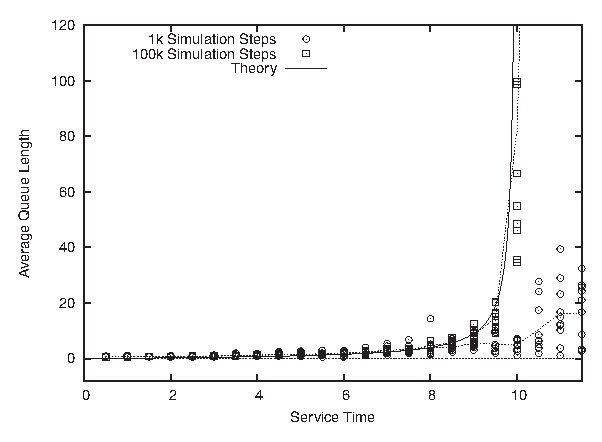
\includegraphics{img/simpy3}}
  \caption{Average queue length as a function of the service time
    for a fixed interarrival time of $t_a = 10$.}
  \label{fig:simpy3}
\end{figure}

Figure \ref{fig:simpy3} shows the results obtained when running the
example program with 1,000 and 100,000 simulation steps. For low
utilization (\ie, short queue lengths), the results from both data
sets agree with each other (and with the theoretical prediction).
However, as the service time approaches the interarrival time, the
short simulation run does not last long enough for the steady state to
form, and so the observed queue lengths are too short.

\index{SimPy!running simulations|)}

\vspace*{-6pt}
\subsection{Summary}

This concludes our tour of discrete event simulation with SimPy. Of
course, there is more to SimPy than mentioned here---in particular,\vadjust{\pagebreak}
there are two additional forms of resources: the \texttt{Store} and
\texttt{Level} abstractions. Both of them not only encapsulate a queue
but also maintain an inventory (of individual items for \texttt{Store}
and of an undifferentiated amount for \texttt{Level}). This inventory
can be consumed or replenished by simulation objects, allowing us to
model inventory systems of various forms. Other SimPy facilities to
explore include asynchronous events, which can be received by
simulation objects as they are waiting in queue and additional
recording and tracing functionality. The project documentation will
provide further details.

\index{simulations!discrete event simulations with SimPy|)}
\index{SimPy|)}

% ============================================================
\section{Further Reading}

\begin{itemize}
\item \cit{A First Course in Monte Carlo}{George S.\ Fishman}{Duxbury
    Press}{2005}
  This book is a nice introduction to Monte Carlo simulations and
  includes many topics that we did not cover. Requires familiarity
  with calculus.

\item \cit{Bootstrap Methods and Their Application}{A.\ C.\ Davison
    and D.\ V.\ Hinkley}{Cambridge University Press}{1997}
  The bootstrap is actually a fairly simple and practical concept, but
  most books on it are very theoretical and difficult, including this
  one. But it is comprehensive and relatively recent.

%\item \cit{Bootstrap Methods}{Michael R. Chernick}{2nd ed., Wiley}{2007} 
%   This book is more of an extensive survey of the existing literature
%   than an original textbook (140 out of 370 pages consist of
%   references!), but it contains some practical hints not easily found
%   elsewhere.

\item \cit{Applied Probability Models}{Do Le Paul Minh}{Duxbury
    Press}{2000}
  The theory of random processes is difficult, and the results often
  don't seem commensurate with the amount of effort required to obtain
  them. This book (although possibly hard to find) is one of the more
  accessible ones.\pagebreak

\item \cit{Introduction to Stochastic Processes}{Gregory F.\
    Lawler}{Chapman \& Hall/CRC}{2006}
  This short book is much more advanced and theoretical than the
  previous one.  The treatment is concise and to the point.

\item \cit{Introduction to Operations Research}{Frederick S.\ Hillier
    and Gerald J. Lieberman}{9th ed., McGraw-Hill}{2009}
  The field of operations research encompasses a set of mathematical
  methods that are relevant for many problems arising in a business or
  industrial setting, including queueing theory.  This text is a
  standard introduction.

\item \cit{Fundamentals of Queueing Theory}{Donald Gross, John F.\
    Shortle, James M.\ Thompson, and Carl M.\ Harris}{4th ed.,
    Wiley}{2008}
  The standard textbook on queueing theory. Not for the faint of heart.

% \item \cit{Stochastic Modeling: Analysis \& Simulation}{Barry L.\
%    Nelson}{Dover Publications}{2010}

\end{itemize}

% stochastic optimization

\index{data analysis!simulations|)}
\index{simulations|)}
